% Instructions to change to html version:
% Comment out:
%  minipage, multicols,columnbreak, mathbf, hrule
% Replace all: \begin{minipage}% \end{minipage} %\begin{multicols}  %\end{multicols} 
% \columnbreak
 %	%% \begin{framed} %\end{framed} %%\hrule
% Replace \mathbf with	\boldsymbol
% Replace $$ with \[ or \]and $ with \( or \)
% Enclose graphics in figure environments and add captions
% 			search \includegraphics
% Re-tag \df environments as sections, subsections, etc.
% Command Line Code to Create html version:
%First: pdflatex -shell-escape filename.tex                                   
%Second, for each figure: inkscape "filename-figure1.pdf" -o "filename-figure1.png"
% Third: htlatex filename.tex "ht5mjlatex.cfg, charset=utf-8" " -cunihtf -utf8"

\documentclass[10pt]{article}

%\usepackage{tikz, pgf,pgfplots,wasysym,array}
%\usepackage{wasysym,array}

\usepackage{amsmath,amssymb}
\usepackage[hidelinks]{hyperref}

\ifdefined\HCode
  \def\pgfsysdriver{pgfsys-tex4ht-updated.def}
\fi 
%\ifdefined\HCode
%  \def\pgfsysdriver{pgfsys-dvisvgm4ht.def}
%\fi 
\usepackage{tikz}
\usetikzlibrary{calc,decorations.markings,arrows}
\usepackage{pgfplots}

\pgfplotsset{compat=1.12}
\usepackage{myexternalize}
\usetikzlibrary{calc,decorations.markings,arrows}
\usepackage{framed}
\usepackage[none]{hyphenat}

\input{../../../common/1336_header_test.tex}
\begin{document}

\newcommand{\an}{\lbrace a_n \rbrace}

\everymath{\displaystyle}

\renewcommand{\myTitle}{MATH 1336: Calculus III}

\renewcommand{\mySubTitle}{Section 5.1, Part 2: More Fun with Sequences! }%\& Section 8.2: Geometric Series}
%~\hfill Name: \underline{~~~~~~~~~~~~~~~~~~~~~~~~~~~~~~~~~~~~~~~~~~~~~~~}

\lectTitle{\vspace*{-.5in}\myTitle}{\vspace*{.1in}\mySubTitle \vspace*{-.2in}}


\setlength{\columnseprule}{0.4pt}
\setlength{\columnsep}{3em}

%\hspace*{-.8in}%\begin{minipage}{1.25\textwidth}
%\begin{framed}
%\begin{multicols}{2}
\section*{More Sequence Definitions: }
A sequence \(\an\) is \textbf{increasing} for all \(n\geq n_0\) if:\\
 \(a_n < a_{n+1}\) for all \(n\geq n_0\).\\~\\
A sequence \(\an\) is \textbf{decreasing} for all \(n\geq n_0\) if:\\
 \(a_n > a_{n+1}\) for all \(n\geq n_0\).\\~\\
A sequence is called \textbf{monotone} (or \textbf{monotonic}) for all \(n\geq n_0\) if:\\
 it is \textit{either} increasing \textit{or} decreasing for all \(n\geq n_0\).\\

~\\

A sequence is \textbf{bounded above} if there is a number \(M\) such that \(a_n\leq M\) for all \(n\geq 1\).\\~\\
A sequence is \textbf{bounded below} if there is a number \(m\) such that \(m\leq a_n\) for all \(n\geq 1\).\\~\\
If a sequence is bounded above and below, then we call it a \textbf{bounded sequence}.\\~\\
If a sequence is not bounded, it is an \textbf{unbounded sequence}.\\

%\columnbreak



\section*{Monotone Convergence Thm. (MCT):}


\textbf{Every bounded, monotone sequence is convergent.}

%\begin{multicols}{2}
\begin{figure}[!h]
\centering
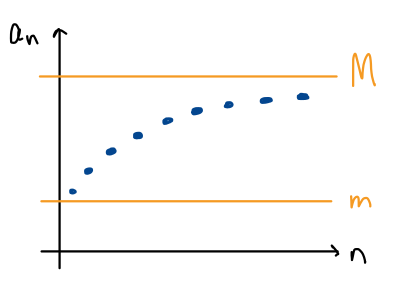
\includegraphics[width=.75\columnwidth]{Ch8s1-MST.png}\\
\caption{Illustration of a bounded increasing sequence, demonstrating the concept of the MCT.}
\end{figure}

\textit{The MCT is important because it is the foundation for proving most of the series tests we will be using later in this chapter!}\\

\textit{(In the previous textbook for this class, this was ``Monotonic Sequence Theorem (MST),'' which may still appear in my notes/solutions as we transition to the new textboook.)}\\

%\end{multicols}

%\hrule
\vspace*{.1in}

\section*{Geometric Sequences:}
 A sequence of the form
\[ a, \quad  ar, \quad  ar^2, \quad  ar^3, \quad  \ldots, \quad  ar^{n-1}, \quad \ldots\]
is called a \textbf{geometric sequence}. \(a\) is the first term, and \(r\) is the \textbf{common ratio}. The n\(^{th}\) term is \(a_n=ar^{n-1}\).\\

A geometric sequence converges if \(-1<r\leq 1\), and diverges otherwise.
\[
\lim_{n\rightarrow \infty} r^n = \left\lbrace\begin{matrix}
0 & \text{if } -1 < r < 1\\
1 & \text{if } r =1
\end{matrix}\right.
\]



%\textbf{Geometric Series:} A series of the form\\
%\( a+ ar+ ar^2+ ar^3+ \ldots+ ar^{n-1}+\ldots = \sum_{n=1}^\infty a r^{n-1}\)\\
%is called a \textbf{geometric series}. \\
%A geometric series converges to \(S=\frac{a}{1-r}\) if \(|r|<1\), and diverges otherwise.

%\end{framed}
%\end{minipage}

\section*{Warm-up Problems:}
Sketch graphs of sequences matching the descriptions below.

\setlength{\columnseprule}{0pt}
%\begin{multicols}{2}
\begin{enumerate}[(a)]

\item a sequence that is decreasing and converges to a finite value

\item a sequence that is bounded that does not converge


\end{enumerate}
%\end{multicols}

\pagebreak

\section*{Examples:}

\begin{enumerate}


\item \textbf{Challenge Problem from last time:}\\
 Determine the convergence of the sequence shown below, where \(n! = 1\cdot 2 \cdot 3 \cdot \ldots \cdot (n-1) \cdot n \)\\
 \(\qquad a_n =\frac{(-3)^n}{n!} \) \\
 
 
 %~\\~\\~\\
 %\\
 %\begin{minipage}{.4\textwidth}
 \begin{figure}[!h]
 \centering
 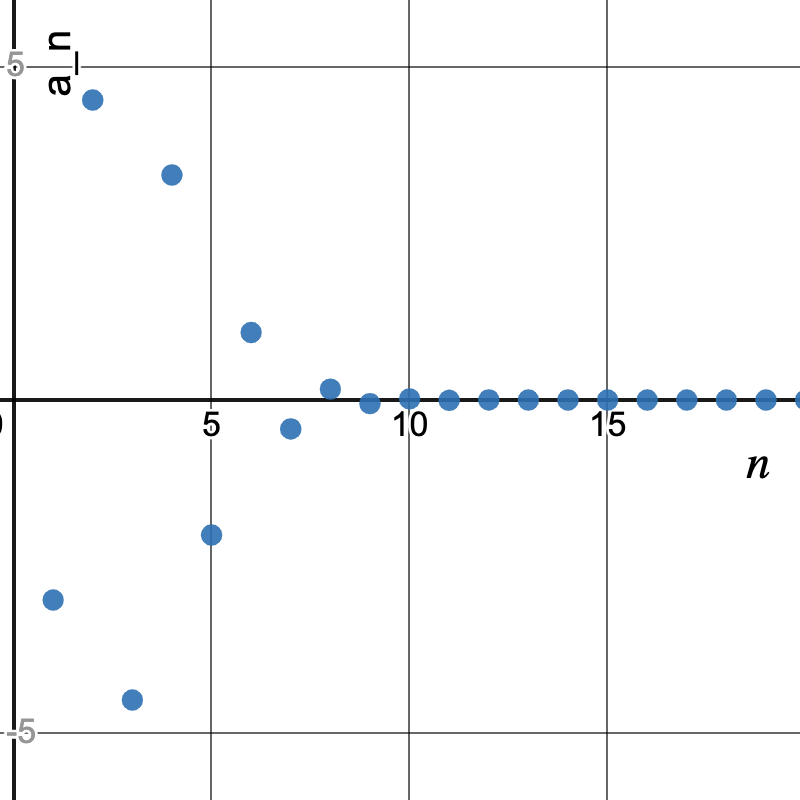
\includegraphics[width=.6\textwidth]{Ch8s1-Challenge-Graph-a.png}
 % }
\caption{(Click \href{https://www.desmos.com/calculator/htfkvazzir}{here} for desmos link)}
 \end{figure}
 %\end{minipage}
 %\begin{minipage}{.6\textwidth}
 

  \textbf{Intuition \& Plan:} If we plot the first several terms of the sequence, we can build intuition that the sequence seems to converge to zero. If we can show that \(\lim_{n\rightarrow\infty} |a_n| = 0 \), then  \(\lim_{n\rightarrow\infty} a_n = 0\).
  ~\\~\\~\\
  
  \textbf{Today's Follow-up Question:} Consider the sequence  \( |a_n | =\frac{3^n}{n!} \).\\
 What, if anything, does the MCT say about this sequence? Can it help us determine the convergence of the original sequence?
  \vspace*{1in}
 %\end{minipage}
 

 


\vfill

%\vfill

\item Determine whether the sequence converges or diverges. If it converges, find the limit.\\
\(\qquad b_n = \ln(3n^2+1) - \ln(n^2-4)\)


\vfill



%\item Determine whether the geometric series is convergent or divergent. If it is convergent, find its sum.
%
%\begin{multicols}{2}
%\begin{enumerate}
%\item \(2+6+18+54+162+\ldots\)
%\item \(2+1+\frac{1}{2}+\frac{1}{4}+\frac{1}{8}+\frac{1}{16}+\ldots\)
%\end{enumerate}
%\end{multicols}
%\vfill

\end{enumerate}

\pagebreak

\section*{Problems for Group Work:}


%\subsection*{Sequence Problems:}

Is the sequence increasing, decreasing, or not monotone? \\
Is the sequence bounded?\\
Does the sequence converge or diverge?
%\begin{multicols}{2}
\begin{enumerate}
\item \(\qquad c_n = 4\left(\frac{-1}{3}\right)^n\)\vfill
\vspace*{1.5in}
\item \(\qquad d_n = 6^n\)\vfill
\vspace*{1.5in}
\item \(\qquad b_n = n+\frac{1}{n}\)\vfill
\vspace*{1.5in}
\item \(\qquad a_n = \frac{2n-3}{3n+4}\)\vfill
\vspace*{1.5in}
\end{enumerate}
%\end{multicols}

The following sequences are geometric. Identify the common ratio, \(r\). Does the sequence converge or diverge?
%\begin{multicols}{2}
\begin{enumerate}
\addtocounter{enumi}{4}
\item
 \[
2, \quad 6, \quad 18, \quad 54, \quad 162, \quad \ldots
\] \label{geo1}

\item
\[
2, \quad 1, \quad \frac{1}{2}, \quad \frac{1}{4}, \quad \frac{1}{8}, \quad \frac{1}{16}, \quad \ldots
\]\label{geo2}




\end{enumerate}
%\end{multicols}

\vfill

\subsection*{Transition Question:}
What do you think will happen if we add up all of the (infinitely many) terms of the sequences shown in problems \ref{geo1} \& \ref{geo2}? 

%\textit{Hint:} Write out the sequence of partial sums for each sequence: \(s_1 = a_1, s_2 = a_1+a_2, s_3 = a_1+a_2+a_3,\ldots\)

%\subsection*{Geometric Series Problems:}
%Determine whether the geometric series is convergent or divergent. If it converges, find its sum.
%\begin{enumerate}
%\addtocounter{enumi}{4}
%\item \( \frac{1}{3}+\frac{1}{27}+\frac{1}{243}+\ldots\)\vfill
%\item \(\sum_{n=1}^\infty	\frac{3^n}{\pi^{n+1}}\)\vfill
%
%
%\end{enumerate}


\end{document}
